\chapter{Appendices for Chapter \ref{ch:Komar2015}}
\label{app:Komar2015}


\section{Local entangling errors}
The initial GHZ state is never perfect due to a series of imperfections in the
implementation. Here, we analyze the main errors responsible for lowering the
initial fidelity $F_\mathrm{local} = [1+\exp(-\eps_\mathrm{local})]/2$ of the GHZ
state of $n$ atoms, created via the conditional dressing scheme,  described in
the main article. We assume the following errors to be independent and small,
and we approximate $\eps_\mathrm{local}$ with the sum
of the individual errors, $\sum_j \eps_j$. We evaluate the errors for a 2D
square lattice filled in a circular region and a 3D cubic lattice filled in a
spherical region (both of radius $R$). Where there is
a difference between the two cases, we give both results.
 
\subsection{Imperfect blockade}
\label{sec:imperfect_blockade}
If the blockade between the levels $r_1$ and $r_2$, $\Delta_{12}$, is not large
enough, the dressing happens even if $r_2$ is populated by a single
atom. Here, we analyze the effect of this imperfection.

The relevant part of the full Hamiltonian of the system during dressing is
\bal
	H &=& \frac{\Omega}{2}\sum_k \left(\ket{r_1}_k\bra{g}_k + \mathrm{h.c.}\right)
	+ \Delta\sum_k \ket{r_1}_k\bra{r_1}_k \\
	&& +\sum_k\sum_{j\neq k}
	\Delta_{j,k}\ket{r_1}_k\bra{r_1}_k\ket{r_2}_j\bra{r_2}_j,
\eal
where $\Omega$ and $\Delta$ are the Rabi frequency and the detuning of the
dressing field, and $\Delta_{j,k} = C_{12}^{(3)}/(\hbar |\br_j - \br_k|^3)$ is
the shift due to dipole-dipole interaction. 
After adiabatically eliminating the level $r_1$, we can write the effective
Hamiltonian as $H_\mathrm{eff} = \sum_k H_k \ket{g}_k\bra{g}_k$, where
\bel
	H_k = -\frac{\Omega^2}{4\Delta} + \sum_{j\neq k}
	\left(\frac{\Omega^2}{4\Delta} - \frac{\Omega^2}{4(\Delta +
	\Delta_{j,k})}\right)\ket{r_2}_j\bra{r_2}_j,
\eel
where we also restricted the Hilbert space to at most one $r_2$ excitation.

Ideally, starting from 
\bel
	\Big(\ket{1_s} + \ket{1_{r2}}\Big)\Big(\ket{g} + \ket{f}\Big)^{\otimes
	(n-1)},
\eel
(where $\ket{1_x} = \sum_j\ket{x}_j/\sqrt{n}$ for $x=s,r_2$),
after time $t = 4\pi\Delta/\Omega^2$, the part
of the wavefunction with no $r_2$ excitaion picks up a $\pi$ phase, 
\bel
	\ket{1_s}\Big(e^{-i\pi}\ket{g} + \ket{f}\Big)^{\otimes (n-1)},
\eel
while the part
where $r_2$ is present is unchanged, or
picks up a small and uniform phase $\phi_0$,
\bel
	\ket{1_{r2}}\Big(e^{i\phi_0}\ket{g} + \ket{f}\Big)^{\otimes (n-1)}.
\eel

In reality, however, dephasing between the different terms of the superposition
occurs. If the system starts from
\bel
	\ket{\Psi_0} = \frac{1}{\sqrt{n}}\sum_j\ket{r_2}_j \bigotimes_{k\neq
	j}\left(\frac{\ket{g}_k + \ket{f}_k}{\sqrt{2}}\right),
\eel
the effective Hamiltonian evolves it into 
\bel
	\ket{\Psi_t} = \frac{1}{\sqrt{n}}\sum_j \ket{r_2}_j
	\bigotimes_{k\neq j} \left(\frac{e^{i\phi_{j,k}}\ket{g}_k +
	\ket{f}_k}{\sqrt{2}}\right),
\eel
up to an overall phase, where $\phi_{j,k} = \pi\Delta/(\Delta + \Delta_{j,k})$,
while the target state is
\bel
	\ket{\Psi_\mathrm{target}} = \frac{1}{\sqrt{n}}\sum_j \ket{r_2}_j
	\bigotimes_{k\neq j} \left(\frac{e^{i\phi_0}\ket{g}_k +
	\ket{f}_k}{\sqrt{2}}\right),
\eel
with an appropriately chosen $\phi_0$. The fidelity of $\Psi_t$ with respect to
$\Psi_\mathrm{target}$ is
\bel
	F = |\ev{\Psi_\mathrm{target}|\Psi_t}|^2 = \left|\frac{1}{n}\sum_j
	\prod_{k\neq j} \frac{1 + e^{i(\phi_{j,k}-\phi_0)}}{2}\right|^2.
\eel
Assuming $|\phi_{j,k} - \phi_0| \ll 1$, and using
\bel
	\frac{1 + e^{ix}}{2} \approx \exp\left[-\frac{x^2}{4} +
	i\frac{x}{2}\right],\qquad \mathrm{for}\quad x\ll 1
\eel
we can write
\bel
	F = \left|\frac{1}{n}\sum_j \left(e^{i\sum_k \frac{\phi_{j,k}-\phi_0}{2}}
	\times e^{-\sum_k\frac{(\phi_{j,k}-\phi_0)^2}{8}}\right)\right|^2.
\eel
We approximate
\bel
	\sum_k (\phi_j,k - \phi_0)^2 \approx n
	\mathrm{Var}\left(\phi_{j,k}\right),
\eel
where the variance is taken over all pairs of $(j,k)$, and we take it out of the
summation to get
\bel
	F \approx \left|\frac{1}{n}\sum_je^{i\sum_k
	\frac{\phi_{j,k}-\phi_0}{2}}\right|^2
	e^{-\frac{n}{4}\mathrm{Var}(\phi_{j,k})}.
\eel
Using the notation,
$\psi_j := \sum_{k\neq j} \phi_{j,k}$, we can write and approximate the first
term as
\bel
	\left|\frac{1}{n}\sum_je^{i\psi_j/2}\right|^2 \approx
	e^{-\frac{1}{4}\mathrm{Var}(\psi_j)},
\eel 
where the variance is taken over all $j$, and we write the total fidelity as
\bel
	F \approx \exp\left[-\frac{1}{4}\mathrm{Var}(\psi_j) -
	\frac{n}{4}\mathrm{Var}(\phi_{j,k})\right] =: e^{-\eps_1}.
\eel

In section \ref{sec:calc_varPhi_jk} and section \ref{sec:calc_varPsi_j}, we
evaluate the above variances for a circular 2D and spherical 3D cloud of radius
$R$, and average density of $a^{-2}$ and $a^{-3}$, respectively. Plugging in the
results of \refeq{eq:Var_phi_jk_2D}, (\ref{eq:Var_phi_jk_3D}) yields
\bal
\label{eq:f1}
	\eps_1 &=& \frac{1}{4}\left[\mathrm{Var}(\psi_j) + n
	\mathrm{Var}(\phi_{j,k})\right]
	\\
	&=&
	\left(\frac{\hbar a^3 \Delta}{C_{12}^{(3)}}\right)^2 \times
	\left\{
		\begin{array}{ll}
			0.0209\, n^5 + 0.156\, n^4 & \quad \mathrm{(2D)}\\
			0.0320\, n^4 + 0.273\, n^3 & \quad \mathrm{(3D)}
		\end{array}
	\right.
	\nonumber
\eal 

\subsection{Decaying Rydberg states}
During dressing, there is an average number of
$n(\Omega/(2\Delta))^2$ Rydberg excitations present at level $r_1$ in the
ensemble.
Any decay or dephasing of $r_1$ Rydberg state then results in the loss of fidelity,
\bel
\label{eq:f2}
	\eps_2 \approx \gamma_1 t \times n \left(\frac{\Omega}{2\Delta}\right)^2 =
	\pi n\frac{\gamma_1}{\Delta},
\eel
where $\gamma_1$ is the total rate of loss (environment induced decay and
dephasing) from the Rydberg level $r_1$, and $t$ is assumed to take the optimal
value, $t = 4\pi\Delta/\Omega^2$.

In the same time, in the other part of the wavefunction, there is exactly one
$r_2$ excitation. If this decays and dephases with rate $\gamma_2$, then  the
fidelity error due to this is
\bel
\label{eq:f3}
	\eps_3 \approx \gamma_2 t = 4\pi \frac{\Delta\gamma_2}{\Omega^2},
\eel
where, again, we used that $t = 4\pi \Delta/\Omega^2$.

\subsection{Rydberg interaction induced broadening}
Although the Rydberg-Rydberg interaction is assumed to be strong, which makes
single-to-double excitations off-resonant, the external laser field can easily
drive Raman transitions between different single excitations states.
Let us define the following states
\bal
	\ket{j} &:=& \sigma_j\+ \ket{gg\ldots g},\qquad\mathrm{where}\quad \sigma\+_j =
	\ket{r_1}_j\bra{g}_j,
	\\
	\ket{S} &:=& \frac{1}{\sqrt{n}}\sum_j \ket{j},
	\\
	\ket{j,k} &:=& \sigma_j\+ \sigma_k\+ \ket{gg\ldots g} = \sigma_j\+ \ket{k} =
	\sigma_k\+ \ket{j}, \quad \mathrm{for}\quad j < k,\qquad
\eal
for $j,k\in \{1,2\ldots n\}$, indexing the atoms in the ensemble.

The full Hamiltonian of the system during the dressing is $H_\mathrm{full}
= \sum_{j=1}^n H_j$, where
\bal
	H_j &=&  \Delta\sigma_j\+ \sigma_j + \frac{\Omega}{2}\big(
	\ket{r_1}_j\bra{g}_j + \mathrm{h.c.}\big)
	\nonumber\\
	&& +
	\sum_{k>j} \Delta_{j,k} \sigma_j\+\sigma_j \sigma_k\+
	\sigma_k.
\eal
It contains a Rydberg-Rydberg interaction term, whose strength,
$\Delta_{j,k} = \Delta_{rr}(|\br_j - \br_k|)$ depends on the
distance between atoms $j$ and $k$. In the subspace of single and double
excitations, $\mathrm{Span}\{\ket{j}, \ket{j,k}\}$, $H_j$ is equivalent to
\bel
	\sum_{k>j} (\Delta + \Delta_{j,k}) \ket{j,k}\bra{j,k} +
	\frac{\Omega}{2}\sum_{k>j} \big( \ket{j}\bra{j,k} + \mathrm{h.c.} \big),
\eel
which is partially depicted on \reffig{fig:coupling 1,2}.

If all Rydberg shifts are large compared to
$\sqrt{n}\Omega$, then the double excitation probability is small, and the
dynamics is well described by the following effective Hamiltonian, $H_\mathrm{eff} = \sum_j
H_{\mathrm{eff}, j}$, where 
\bel
\label{eq:H_eff}
	H_{\mathrm{eff},j} = \Delta_j \ket{j}\bra{j} + \sum_{k>j}
	\frac{\Omega_{j,k}}{2} \big( \ket{j}\bra{k} + \mathrm{h.c.} \big),
\eel
where $\Delta_j = -\sum_{k\neq j}\frac{\Omega^2}{4(\Delta_{j,k} + \Delta)}$, and    
$\Omega_{j,k} = -\frac{\Omega^2}{2(\Delta_{j,k} + \Delta)}$.
\begin{figure}[h]
\centering
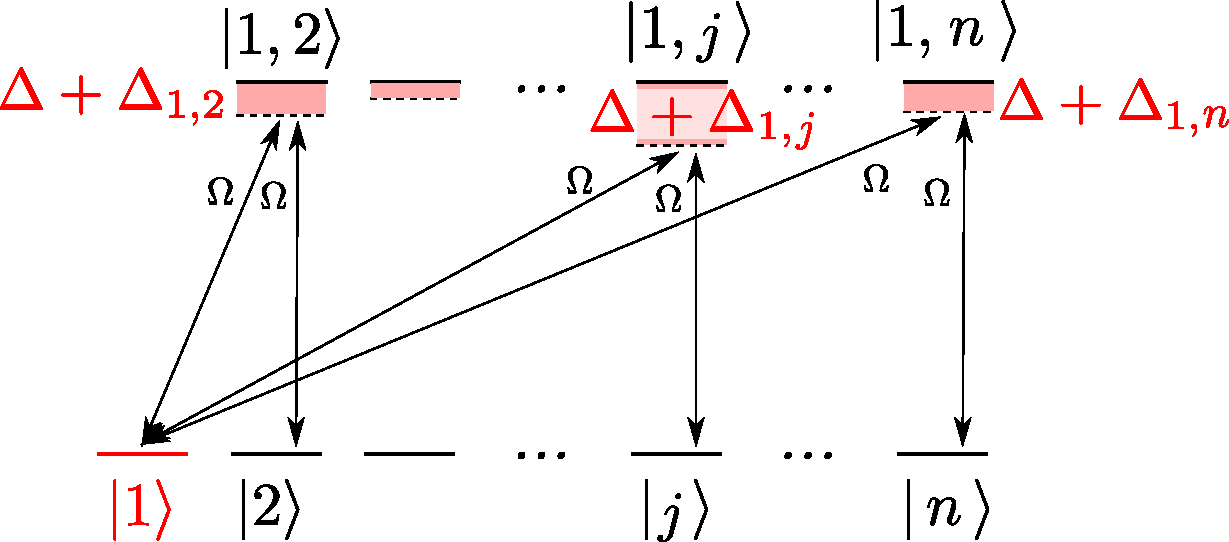
\includegraphics[width=0.80\textwidth]
{./figs_Komar2015/coupling_1_2_smalln_only1.pdf} 
\caption
[Coupling through doubly excited states]
{
\label{fig:coupling 1,2}   
Different single excitation states ($\ket{j} = \sigma_j\+ \ket{gg\dots g}, \; j
= 1,2,\dots n$) are resonantly coupled to each other through a Raman-transition
via double excited states ($\ket{j,k} = \sigma_j\+\sigma_k\+\ket{gg\dots g},\;
j < k$). The effective coupling strengths depend on the detuning of the
intermediate level, and results in an inhomogeneous broadening. (The figure
shows only the double excited states that couple to $\ket{1}$.)}
\end{figure}

The two terms in \refeq{eq:H_eff} have different effects. The first
term describes inhomogeneous broadening. Due to this effect, the fidelity of the
symmetric state $\ket{S}$ decreases over time, $t$, as
\bel
	\left|\Ev{S\left| e^{-i\sum_j\Delta_jt
	\ket{j}\bra{j}}\right|S}\right|^2 = \left|\frac{1}{n}\sum_j
	e^{-i\Delta_j t}\right|^2 \approx e^{-t^2 \mathrm{Var}(\Delta_j)}.
\eel
Since the expected number of excitations during the dressing pulse is small,
$\sim n[\Omega/(2\Delta)]^2$, we can write the error as $\eps_{4a} \approx
n[\Omega/(2\Delta)]^2 t^2 \mathrm{Var}(\Delta_j)$.


The effect of the second term in \refeq{eq:H_eff}, couples
different single-excitation states coherently. We put an upper bound of the
effect of this term by analyzing it without the detuning effect of the
$\Delta_j$ terms. Let us define the following states,
\bel
	\ket{\tilde j} := \left(1-\frac{1}{n}\right)^{-1/2}\left( \ket{j} -
	\frac{1}{\sqrt{n}}\ket{S} \right),
\eel
for $j = 1,2,\dots n$.
These states are all orthogonal to $\ket{S}$, normalized, and span an $n-1$
dimensional space, therefore they are overcomplete by a factor of $n/(n-1)$, and
they are also almost orthogonal to each other:
$
	|\ev{\tilde j | \tilde k}| =
	\frac{1}{n} + \frac{1}{n^2} = \OO(1/n).
$
Let us imagine starting the system in
$\ket{S}$, and observing the probability accumulating in all the other states
$\ket{\tilde j}$. The time evolution of the amplitudes, $\tilde c_j$, dictated
by the Heisenberg equations, can be approximated as
\bal
	\frac{d}{dt}\tilde c_j(t) &=& -i\ev{\tilde j| H_{\mathrm{eff},\Omega} |S} c_s(t)
	+ \OO(\tilde c_k(t)) \nonumber\\
	&\approx& -i\ev{\tilde j | H_{\mathrm{eff},\Omega}| S}c_s(0),
	\nonumber\\
	\tilde c_j(t) &\approx& -it\ev{\tilde j| H_{\mathrm{eff},\Omega} |S}c_s(0),
\eal
where, $|c_s(0)|^2 \approx n (\Omega/(2\Delta))^2$, and $H_{\mathrm{eff},\Omega}
= \sum_{j,k>j} \Omega_{j,k}(\ket{j}\bra{k} + \mathrm{h.c.})$. The conditional
probability accumulating in $\ket{\tilde j}$ is
\bal
	\frac{P_j(t)}{|c_s(0)|^2} &\approx& t^2 \left|\ev{\tilde
	j|H_{\mathrm{eff},\Omega}|S}\right|^2 \nonumber\\
	&\approx& 
	t^2\left|\sum_k \frac{1}{\sqrt{n}}\left(\frac{\Omega_{j,k}}{2} -
	\frac{1}{n}\sum_l \frac{\Omega_{l,k}}{2}\right)\right|^2 \nonumber\\
	&=& t^2\frac{1}{n} \left|\Delta_j - \frac{1}{n}\sum_l \Delta_l \right|^2,
\eal
where we used that $\sum_{k\neq j}\Omega_{j,k}/2 = \Delta_j$.
The total conditional probability of leaving the
symmetric state $\ket{S}$ is
\bal
	\frac{P(t)}{|c_S(0)|^2} &\approx& t^2 \frac{1}{n} \sum_j \left|\Delta_j -
	\frac{1}{n}\sum_l \Delta_l\right|^2 = t^2\mathrm{Var}(\Delta_j),\quad
\eal
and the total error is $\eps_{4b} = P(t) = n[\Omega/(2\Delta)]^2 t^2
\mathrm{Var}(\Delta_j)$. This is identical to the error originating from the
$\Delta_{jk}$ term of \refeq{eq:H_eff}. We approximate the effect of these two
errors by adding them, giving
\bel
	\eps_{4a} + \eps_{4b} = 
	\frac{n}{2}\left(\frac{\Omega}{\Delta}\right)^2 t^2 \,\mathrm{Var}(\Delta_j).
\eel

We evaluate the variance of $\Delta_j$ in section \ref{sec:calc_varDelta_j} for
both the 2D and the 3D case.
The result is given in \refeq{eq:varDelta_j_2D} and (\ref{eq:varDelta_j_3D}).
Plugging the result in, and using that $t = 4\pi\Delta/\Omega^2$, we can write
the error as
\bal 
\label{eq:f4}
	&&\eps_4 \approx \eps_{4a} + \eps_{4b} = 
	\left\{
	\begin{array}{ll}
	0.0312\, n^9
	\left(\frac{\hbar a^6\Omega}{C_{11}^{(6)}}\right)^2 & \mathrm{(2D)}
	\\
	0.172\, n^7 \left(\frac{\hbar a^6\Omega}{C_{11}^{(6)}}\right)^2 &
	\mathrm{(3D)}
	\end{array}
	\right.
	\qquad
\eal
where $a$ is the lattice constant of the 2D (3D) optical lattice holding the
atoms, and $C_{11}^{(6)}$ is the coefficient of the van der Waals interaction
between two atoms excited to $r_1$ level.


\section{Non-local entangling errors}
Our protocol requires $K-1$ links to be set up between $K$ clocks. 
We denote the fidelity of a single connection by $F_\mathrm{non-local} =
[1+\exp(-\eps_\mathrm{non-local})]/2$,  and we approximate $\eps_\mathrm{non-local}$
with the  sum of individual errors $\sum_i \eps_i$, detailed below.

\subsection{Imperfect blockade}
When exciting a single collective excitations, imperfect self-blockade can
result in leakage into double excited states. The probability of this can be
exponentially reduced by applying a smooth driving pulse. E.g., in case of a
Gaussian pulse of width $\tau$, and area $\pi$, exciting the $g
\rightarrow r_1$ transition is expected to be blocked when $r_2$ is populated, 
but it succeeds with probability $P_\mathrm{double}$,
\bel
	P_\mathrm{double} \approx \frac{\pi^2}{4}
	\exp\left[-\frac{(\Delta_{12}\tau)^2}{2}\right],
\eel
where $\Delta_{12} = C^{(3)}_{12}/(\hbar (2R)^3)$ is the minimal energy
shift in the ensemble due to the interaction of two atoms, one in $r_1$ and one
in $r_2$.
A detailed analysis of how different pulses affect the
transition probability can be found in \cite{Conover2011}. $P_\mathrm{double} \ll
1$ requires
\bal
\label{eq:tau}
	&&\tau \leq \frac{\sqrt{2}}{\Delta_{12}} = 
	\left\{
	\begin{array}{ll}
	2 n^{3/2} \frac{\hbar a^3}{C^{(3)}_{12}} & \mathrm{(2D)} 
	\\
	2.7\, n  \frac{\hbar a^3}{C^{(3)}_{12}} & \mathrm{(3D)}
	\end{array}
	\right.
\eal 
in order to be small compared to the other errors.

\subsection{Rydberg state decay}
The $g\rightarrow r_1$ transition is driven with a pulse of duration $\tau$,
during which the $r_2$ level has a single excitation, which decays with rate
$\gamma_2$. The resulting error contribution, after all four photon pulses have
been generated, is
\bal
\label{eq:f5}
	&&\eps_5  = 4 \gamma_1 \tau = 
	\left\{
	\begin{array}{ll}
	8 n^{3/2} \frac{\hbar a^3 \gamma_1}{C_{12}^{(3)}} & \mathrm{(2D)}
	\\
	10.8\, n \frac{\hbar a^3 \gamma_1}{C_{12}^{(3)}} & \mathrm{(3D)}
	\end{array}
	\right.
\eal
where we used the expressions for $\tau$ from \refeq{eq:tau}.

\subsection{Photon propagation and detection errors}
The pairs of photons can get lost in the fiber during propagation and the
detection process (which is limited to 50\% for time-resolving detectors,  and
25\% for non-time-resolving ones). The two-photon heralding, however, detects
both of these errors. The remaining error comes from dark-counts of the
detectors. This affects a single link with the error
\bel
\label{eq:f6}
	\eps_6 \approx 4 \gamma_\mathrm{dark}
	T_\mathrm{detect} = \gamma_\mathrm{dark} \frac{20}{n \gamma_e},
\eel
where $\gamma_\mathrm{dark}$ is the dark count rate of the detectors,
 $T_\mathrm{detect}$ (chosen such that a properly timed detector would have a
 chance to catch $1 -e^{-5} >  99\%$ of each photon) is the ``open time'' of the
 detector, and $\gamma_{e}$ is the spontaneous emission lifetime of the
 $\ket{e}\rightarrow \ket{f}$ transitions.
 The factor of $n$ is due to the bosonic enhancement of the said transition, and
 the factor of 4 is because four pulses are used in each connection.


\subsection{Memory loss}
During the creation step of each link, the state $\ket{s}$ is used as memory.
On average, every link relies on one $s$ qubit. The time it takes to attempt the
creation of a link is $\sim 2L/c$, the time it takes for a light pulse to do a
round-trip between two stations.
During this time, quantum information is stored in qubit $s$, which is subject
decoherence happening at a rate $\gamma_s$.
The infidelity of the link originating from this error is
\bel
\label{eq:f7}
	\eps_7 = 4\frac{2L}{c}	\gamma_s.
\eel
State $\ket{f}$ is assumed to be a long-lived clock state, its decoherence rate
is negligible.

% In order to minimize the time each $s$ qubit is used to store quantum
% information, we assume that each site does the following. After attempting
% entanglement with the neighbors (using the $f$ qubit for the left neighbor, and
% the $s$ qubit for the right neighbor), four things can happen. If none of them
% or both of them succeeds the protocol  tries or performs a connection step right
% away. If only the left link succeeds then that is kept, and the right one
% (supported by the $s$ qubit) needs to be retried. If, however, the left one
% did not succeed but the right one does, then the site performs a swap between
% the $f$ and $s$ qubits, and further attempts to connect the left link will use
% the (no empty) $s$ qubit.

\subsection{Imperfect branching ratios}
Bosonic enhancement makes the excited atom in state $\ket{e}$ decay
preferentially to $\ket{g}$, and emit a photon directly to the spatial mode
$\bk_e$, where $\bk_e$ is the spatial frequency of the collective mode $e$.
However, in the implementation with Yb atoms (discussed in Section
\ref{sec:Implementation}), the decay channel to $\ket{g}$ has a branching ratio
of $\zeta = 0.64$. The total probability of decay through all other channels is
\bel
\label{eq:f8}
	\eps_8 = 4 \frac{\gamma_{\mathrm{not}\,f}}{\gamma_\mathrm{tot}} \approx
	4\frac{1-\zeta}{n\zeta + 1-\zeta} \sim \frac{2}{n},
\eel
where $n\,(\gg 1)$ is the number of atoms in a single ensemble.



\section{Implementation with Yb}
\label{sec:Implementation}
We imagine using the lower levels of neutral Yb for our protocol,  $\ket{g} =
\ket{6s6p({}^3P_0)}$, $\ket{f} = \ket{6s^2({}^1S_0)}$, $\ket{s} =
\ket{6s6p({}^3P_2)}$ and $\ket{e} = \ket{5d6s({}^3D_1)}$, and two Rydberg
levels $\ket{r_1} = \ket{6s\tilde n s({}^1S_0)}$ and $\ket{r_2} =
\ket{6s\tilde n p_{m=+1}({}^1P_1)}$ with the same principle
quantum number $\tilde n$ for high-energy state. In the case of the 2D
lattice, we set the quantization axis perpendicular to the plane in which the
atoms reside, this way the dipole-dipole interaction between two atoms, one in $\ket{r_2}$ and the other in $\ket{r_1}$,
depends only on their separation, $|\br_1 - \br_2|$. In the case of the 3D
lattice, we rely on the overwhelming strength of the Rydberg interaction to
produce reliable blockade even between atoms in different horizontal planes.

\subsection{Rydberg lifetimes}
We use the measured values from \cite{Fang2011}, and extrapolate the
inverse lifetimes of the Rydberg states
\bel
	\gamma_1\approx\gamma_2 = \gamma = \frac{8.403\times
	10^8~\mathrm{Hz}}{(\tilde n-4.279)^3}
\eel
where $\tilde n$ is the principle quantum number of the Rydberg orbit. Although
the measurement was carried out at $300~\mathrm{K}$, the
contribution of the black body radiation is negligible even at this temperature.
Furthermore, the photoionization rate in a trapping field with
$10^4~\mathrm{W}/\mathrm{cm}^2$ intensity is also more than one order of magnitude
smaller.


\subsection{Self-blockade, $\Delta_{11}$}
The long-range interaction between two $r_1$ atoms at a distance $R$ is
dominated by the van der Waals potential,
\bel
\label{eq:Delta_{11}(a)} 
	\Delta_{11}(R) = \frac{C_{11}^{(6)}}{\hbar R^6},
\eel
where $C_{11}^{(6)}$ strongly depends on the principle quantum number $\tilde
n$. We use results from \cite{Topcu2015}, and extrapolate the $C_{11}^{(6)}$
coefficient to high principle quantum numbers with the following formula,
\bel
	C_{11}^{(6)} = (-0.116 + 0.0339\, \tilde n) \,\tilde n^{11}\,
	\mathrm{a.u.}
\eel
where the a.u. stands for atomic units, $E_h a_0^6 = 9.573\times
10^{-80}~\mathrm{Jm}^6$, where $E_h$ is the Hartree energy and $a_0$ is the Bohr
radius.

% 
% The long-range interaction between two $r_2$ atoms at a distance $a$ is
% dominated by the van der Waals potential,
% \bel
% \label{eq:Delta_{22}(a)}
% 	\Delta_{22}(a) = \frac{C_{22}^{(6)}}{\hbar a^6},
% \eel
% where $C_{22}^{(6)}$ strongly depends on the principle quantum number $\tilde
% n$. This is shown on \reffig{fig:C_{6,22}}, where we plot $C^{(6)}_{22}$, as a
% function of $\tilde n$ in atomic units. (From [REF: Turker's paper])
% \begin{figure}[h]
% \centering
% \includegraphics[width=0.5\textwidth]{./figs/C6ss_plot.pdf}
% \caption{
% \label{fig:C_{6,22}} Absolute value of the van der Waals coefficient,
% $|C_{22}^{(6)}|$, in atomic units $(9.57\times 10^{-80}\,\mathrm{Jm}^6)$, as a
% function of the principle quantum number of the Rydberg orbit $\tilde n$.} 
% \end{figure}
% 

\subsection{Cross-blockade, $\Delta_{12}$}
The long-range interaction between an $r_1$ and an $r_2$ atoms at a distance $R$
is dominated by the dipole-dipole interaction. We assume that the atoms are
confined in the $xy$ plane, and  because the $6s\tilde n p_{m=+1}$ state is
polarized in the $z$ direction, the interaction strength is independent of the
relative direction of one atom to the other.
\bel
\label{eq:Delta_{12}(a)}
	\Delta_{12}(R) = \frac{C_{12}^{(3)}}{\hbar R^3},
\eel
where $C_{12}^{(3)}$ depends strongly on the principle quantum number $\tilde
n$. We use results from \cite{Topcu2015}, and extrapolate the $C_{12}^{(3)}$
coefficient to high principle quantum numbers with the following formula,
\bel
	C_{12}^{(3)} = (0.149 + 0.00077\, \tilde n) \,\tilde n^{4}\,
	\mathrm{a.u.}
\eel
where the a.u. stands for atomic units, $E_h a_0^3 = 6.460\times
10^{-49}~\mathrm{Jm}^3$.


% \subsection{Shifts relative to linewidth}
% We assume trapping the atoms in an optical square lattice with a trapping laser
% of wavelength $551.5\,\mathrm{nm}$, which results in a lattice constant $a =
% 275.75\,\mathrm{nm}$. The frequency shifts between two neighboring atoms due to
% the Rydberg interactions are $\Delta_{11}(a)$ and $\Delta_{12}(a)$ from
% \refeq{eq:Delta_{11}(a)}, \refeq{eq:Delta_{12}(a)}.  We are interested in the
% shifts relative to the linewidth, and we define
% \bal
% 	\delta_{11} &=& \frac{\Delta_{11}(a)}{\gamma} =
% 	\frac{\left|C_{11}^{(6)}\right|}{a^6\hbar \gamma},
% 	\\ 
% 	\delta_{12} &=& \frac{\Delta_{12}(a)}{\gamma} =
% 	\frac{\left|C_{12}^{(3)}\right|}{a^3\hbar \gamma}.
% \eal
% We plot $\delta_{11}$ and $\delta_{12}$ as a function of $\tilde n$  on
% \reffig{fig:deltas}.
% \begin{figure}[h]
% \centering
% \includegraphics[width = 0.5\textwidth]{./figs/deltas_plot.pdf}
% \caption{
% \label{fig:deltas}
% Normalized frequency shifts between neighboring atoms in an optical lattice with
% lattice constant $a = 275.75\,\mathrm{nm}$, if they are both in $r_1$ state
% ($\delta_{11}$), and if one of them is in $r_1$ and the other in $r_2$ state
% ($\delta_{12}$), as a
% function of the principle quantum number of the Rydberg orbit $\tilde n$.
% Note that $\delta_{12} \gg
% \delta_{11}$ only for $\tilde n < 25$.}
% \end{figure}

\subsection{Decay rates of lower levels}
The decay rate of $\ket{s} =\ket{6s6p\,,{}^3P_2}$ is $\gamma_s = 
[14.5\,\mathrm{s}]^{-1} = 0.069\,\mathrm{Hz}$. The decay rate of the excited state
$\ket{e} = \ket{5d6s\,,{}^3D_1}$ is $\gamma_e  = [380\,\mathrm{ns}]^{-1} = 
2.63\times 10^6\,\mathrm{Hz}$.


\subsection{Photon channels}
We assume that neighboring stations are $L < 10\,\mathrm{km}$ apart from each
other, we neglect fiber and coupling loss. We further assume that single photon
detectors have a low dark count rate, i.e.
$\gamma_\mathrm{dark}\approx 10\,\mathrm{Hz}$.


\section{Optimization}
The total initial imperfections of a GHZ state with $N$ atoms divided into $K =
N/n$ groups, each containing $n$ atoms, is
\bal
	\eps_\mathrm{tot} &=& (K-1)\eps_\mathrm{non-local}
	+ K \eps_\mathrm{local} \approx -\frac{N}{n}\sum_i \eps_i,
\eal
where the error contributions are from Eq. (\ref{eq:f1}, \ref{eq:f2},
\ref{eq:f3}, \ref{eq:f4}, \ref{eq:f5}, \ref{eq:f6}, \ref{eq:f7},
 and \ref{eq:f8}). 
Independently from the total atom number, $N$, there is an optimal group size,
$n_\mathrm{opt}$, for which $\sum_i\eps_i / n$ is minimal. If the total number of
atoms is increased, it is best to create multiple groups of the same size. Below
we find the optimal values of the parameters $\Omega$, $\Delta$ (the Rabi
frequency and the detuning of the dressing scheme), and $n$ (the size of the
local groups) for fixed values of $\tilde n$ (the principle quantum number of
the Rydberg state) and  $a = 275.75\,\mathrm{nm}$.

Using the following dimensionless variables, $\omega = \Omega / \gamma$,
$\delta = \Delta/\gamma$, $\delta_{11} = \frac{C_{11}^{(6)}}{\hbar a^6
\gamma}$ and $\delta_{12} = \frac{C_{12}^{(3)}}{\hbar a^3\gamma}$, we can write
the error per atom as $E:= \sum_i\eps_i / n = \sum_i e_i$, where the terms
are
\bal
	e_1 &=& 
	\left(\frac{\delta}{\delta_{12}}\right)^2\times 
	\left\{
	\begin{array}{ll}
	0.021\, n^4 + 0.16\, n^3
	 & \mathrm{(2D)}
	\\
	0.032\, n^3 + 0.27\,n^2 & \mathrm{(3D)}
	\end{array}
	\right.
	\\
	e_2 &=& \frac{\pi}{\delta}
	\\
	e_3 &=& \frac{4\pi}{n}\frac{\delta}{\omega^2}
	\\
	e_4 &=& \left(\frac{\omega}{\delta_{11}}\right)^2 \times
	\left\{
	\begin{array}{ll}
	0.031\, n^8
	& \mathrm{(2D)}
	\\
	0.17 \, n^6
	& \mathrm{(3D)}
	\end{array}
	\right.
	\\
	e_5 &=& \frac{1}{\delta_{12}} \times
	\left\{
	\begin{array}{ll}
	8 n^{1/2} & \mathrm{(2D)}
	\\
	10.8 & \mathrm{(3D)}
	\end{array}
	\right.
	\\
	e_6 &=&
	7.6\times 10^{-5}\, \frac{1}{n^2}
	\\
	e_7 &=& 1.8\times 10^{-5}\,\frac{1}{n}
	\\
	e_8 &=& \frac{2}{n^2}
\eal

\subsection{Optimal parameters}
We numerically minimized the sum, $E = \sum_i e_i$, by finding the optimal
values of $\omega, \delta$ and $n$ for every $\tilde n \in [50,150]$. The optimal driving
strength $\omega_\mathrm{opt}$, the optimal
detuning for the dressing field $\delta_\mathrm{opt}$, and  the optimal
number of atoms at a single clock $n_\mathrm{opt}$ are shown on \reffig{fig:opts}. 
\begin{figure}[h] \centering
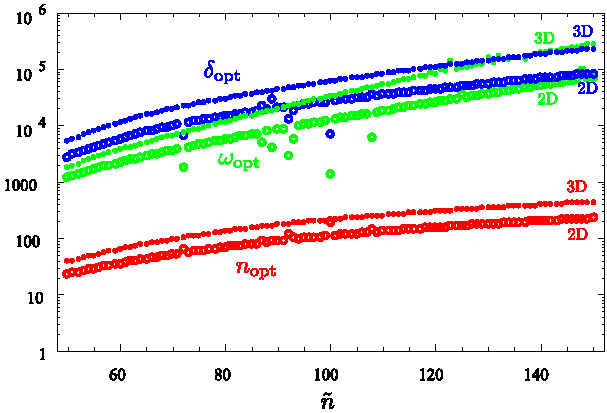
\includegraphics[width=0.8\textwidth]{./figs_Komar2015/n_omega_delta_2d3d.pdf} 
\caption
[Optimal parameter values]
{
\label{fig:opts}
The dressing fields optimal Rabi frequency $\omega = \Omega/\gamma$, detuning
$\delta = \Delta/\gamma$ and the optimal number of atoms in a single clock $n$
is plotted as a function of the principle quantum number of the Rydberg levels
$\tilde n$, for the 2D and 3D setup.}  
\end{figure}

The
minimal error per atom $E_\mathrm{min}$ is shown on
\reffig{fig:E_min}  as a function of $\tilde n$.
\begin{figure}[h]
\centering
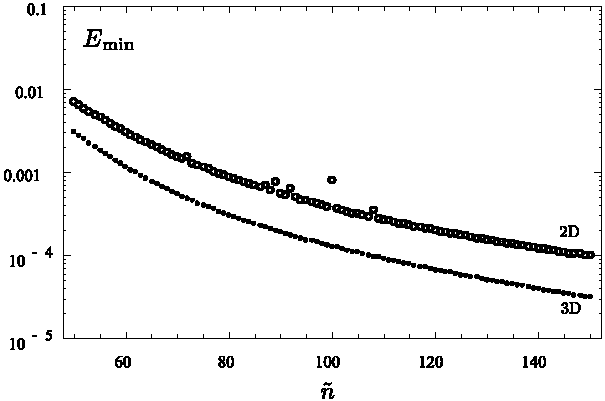
\includegraphics[width=0.8\textwidth]{./figs_Komar2015/Eone_2d3d.pdf}
\caption
[Minimal error per atom]
{
\label{fig:E_min}
The minimized error contribution of a single atom as a function of the principle
quantum number of the Rydberg levels $\tilde n$, for the 2D and 3D setup.}
\end{figure}



\subsection{Comparison of error sources}
We compare the contributions of the different error terms $e_i$ to the total
error per atom, $\sum_i e_i$, for $\tilde n = 120$. At the optimum
(2D: $n_\mathrm{opt} = 154$, $\delta_\mathrm{opt} = 4.40\times 10^4$,
$\omega_\mathrm{opt} = 2.59\times 10^4$, 3D: $n_\mathrm{opt} = 298$,
$\delta_\mathrm{opt} = 10.9\times 10^4$, $\omega_\mathrm{opt} = 8.33\times 10^4$), 
the total error per atom is $E_\mathrm{min} = 
1.99\times 10^{-4}$ (2D), and $0.67\times 10^{-4}$ (3D).
The different error terms contribute to the sum with amounts given in Table
\ref{table:errors_2D} and \ref{table:errors_3D}.
\begin{table}
\centering
\begin{tabular}{|l|c|c|}
\hline
 Errors in 2D ensemble & error per atom & ratio in total\\
\hline
imperfect blockade ($e_1$) & $3.30 \times 10^{-5}$ & 17\%\\
$r_1$ decay ($e_2$) & $7.14 \times 10^{-5}$ & 36\%\\
$r_2$ decay ($e_3$) & $5.36 \times 10^{-6}$ & 3\%\\
inhom. broadening ($e_4$) & $5.36 \times 10^{-6}$ & 3\%\\
$r_2$ decay (non-local) ($e_5$) & $ \sim 10^{-9}$ & $<0.1$\%\\
photon detection ($e_6$) & $ \sim 10^{-9}$ & $<0.1$\%\\
memory error ($e_7$) & $ \sim 10^{-7}$ & $<0.1$\%\\
imperfect br. ratios ($e_8$) & $8.40 \times 10^{-5}$ & 42\%\\
\hline
total error per atom & $1.99 \times 10^{-4}$ & 100\%\\
\hline
\end{tabular}
\caption
[Error budget of 2D setup]
{
\label{table:errors_2D}
The absolute and relative contribution of the different error sources to the
total error per atom at $\tilde n = 120$, $\Delta =
\Delta_\mathrm{opt} = 4.40\times 10^4\,\gamma$, $\Omega = \Omega_\mathrm{opt} = 
2.59\times 10^4\,\gamma$ and $n = n_\mathrm{opt} = 154$.}
\end{table}

\begin{table}
\centering
\begin{tabular}{|l|c|c|}
\hline
 Errors in 3D ensemble & error per atom & ratio in total\\
\hline
imperfect blockade ($e_1$) & $1.41 \times 10^{-5}$ & 21\%\\
$r_1$ decay ($e_2$) & $2.89 \times 10^{-5}$ & 43\%\\
$r_2$ decay ($e_3$) & $6.62 \times 10^{-7}$ & 1\%\\
inhom. broadening ($e_4$) & $6.62 \times 10^{-7}$ & 1\%\\
$r_2$ decay (non-local) ($e_5$) & $ \sim 10^{-10}$ & $<0.1$\%\\
photon detection ($e_6$) & $ \sim 10^{-9}$ & $<0.1$\%\\
memory error ($e_7$) & $ \sim 10^{-8}$ & $<0.1$\%\\
imperfect br. ratios ($e_8$) & $2.26 \times 10^{-5}$ & 34\%\\
\hline
total error per atom & $0.670 \times 10^{-4}$ & 100\%\\
\hline
\end{tabular}
\caption
[Error budget of 3D setup]
{
\label{table:errors_3D}
The absolute and relative contribution of the different error sources to the
total error per atom at $\tilde n = 120$, $\Delta =
\Delta_\mathrm{opt} = 10.9\times 10^4\,\gamma$, $\Omega = \Omega_\mathrm{opt} = 
8.33\times 10^4\,\gamma$ and $n = n_\mathrm{opt} = 298$.}
\end{table}
% To get an idea of how narrow is the optimum, and how each component of the error
% contributes to it, we plot the error terms, each $e_i$ separately, for $\tilde n
% = 120$, as a function of $n$, while using previously determined optimal values for 
% $\omega$ and $\delta$. (We do not optimize them for every choice of $n$.) This
% is shown on \reffig{fig:errors}.
% \begin{figure}[h]
% \centering
% \includegraphics[width=0.48\textwidth]{./figs/errors_xxx.pdf}
% \caption{
% \label{fig:errors}
% Contributions of the different error terms, $e_i$, and the total error
% per atom, $\sum_i e_i$, for principle quantum number $\tilde n = 120$, and $\delta =
% \delta_\mathrm{opt} = 2.02\times 10^4$, $\omega = \omega_\mathrm{opt} =  2.15\times
% 10^3$ for different values of $n$. The global minimum of the sum $\sum_i e_i$ is
% located at $n = n_\mathrm{opt} = 209$. The description of the error terms denoted
% by $e_i$ is given in Table \ref{table:errors}.}
% \end{figure}


\section{Clock precision}

\subsection{Imperfect initialization}
The precision of an atomic clock employing a GHZ state of $N$ clock atoms is
limited by the initial imperfect creation of the GHZ state
described by the fidelity $F_N$ or contrast $c = 2F_N -1$.
We assume that an imperfect creation of the GHZ state result in the density
matrix 
\bel
	\rho_\mathrm{non-pure} = c \ket{\Psi}
	\bra{\Psi}
	 + \frac{1-c}{2}\big(
	\ket{\mathbf{0}}\bra{\mathbf{0}} + \ket{\mathbf{1}}\bra{\mathbf{1}} \big),
\eel
where $\ket{\Psi} = \frac{\ket{\mathbf{0}} + \ket{\mathbf{1}}
}{\sqrt{2}}$, $\ket{\mathbf{0}} = \ket{0}^{\otimes N}$, $\ket{\mathbf{1}} =
\ket{1}^{\otimes N}$, and we assumed that only the relative phase between the
two components of the GHZ state changes to an unknown value,  but no
relaxation happens.

\subsection{Measurement}
After the interrogation time, the two components of the GHZ state pick up a
relative phase $N\phi$. $\ket{\Psi}\rightarrow \ket{\Psi_\phi} =
[\ket{\mathbf{0}} + e^{iN\phi}\ket{\mathbf{1}}]/\sqrt{2}$. Performing a perfect
single-atom $-\pi/2$ rotation around the $y$ axis for all atoms transforms this
into
\bel
	\ket{\Psi'_\phi} = \frac{1}{\sqrt{2^{N+1}}}\sum_{\{q_j\}} \left[1
	+(-1)^{\sum_j q_j} e^{iN\phi}\right] \ket{q_1,q_2, \dots q_N},
\eel
where $q_j\in\{0,1\}$ stands for the state of atom $j$. After this, we 
measure every atom (in the $z$-basis). The probability of any resulting
sequence, $\mathbf{q} = (q_1, q_2, \dots q_N) \in \{0,1\}^{\times N}$, is
\bel
	\PP(\mathbf{q} | \Psi'_\phi) = \frac{1}{2^{N+1}} \left[1 + (-1)^{\sum_j
	q_j} \cos(N\phi) \right],
\eel
and the probability of the parity, $p = \big(\sum_j q_j\big)\mathrm{ mod } 2$, is
\bel
	\PP(p|\Psi'_\phi) = \frac{1 + (-1)^p\cos(N\phi)}{2}, \qquad p\in\{0,1\}.
\eel

On the other hand, these probabilities are different when they are conditioned
on being in the mixed part of the density matrix.
\bel
	\PP(\mathbf{q}|\rho_\mathrm{mixed}) = \frac{1}{2^N}, \qquad
	\PP(p|\rho_\mathrm{mixed}) = \frac{1}{2}
\eel
$\forall \mathbf{q}\in\{0,1\}^{\times N}$ and $\forall p\in\{0,1\}$, where
$\rho_\mathrm{mixed} = [\ket{\mathbf{0}}\bra{\mathbf{0}} +
\ket{\mathbf{1}}\bra{\mathbf{1}}]/2$.

The resulting total probability is the weighted sum of the
two cases,
\bal
	\PP(p|\phi) &=& c\PP(p|\Psi'_\phi) + (1-c)\PP(p|\rho_\mathrm{mixed})
	\quad \\
	&=&
	\frac{1 + c(-1)^p\cos(N\phi)}{2},
\eal
where $c = 2F_N -1$ is the
contrast of the interference fringes.


\subsection{Fisher information}
We rely on inferring the unknown phase $\phi$, from a series of parity
measurements, as described above. The information content  (about $\phi$) of a
single measured value $p$ is quantified by the Fisher information,
\bal
	\mathcal{F}(\phi) &=& \sum_{p\in\{0,1\}} \PP(p|\phi)
	\left[\ln\frac{d}{d\phi} \PP(p|\phi)\right]^2
	\\
	&=& N^2 \frac{\sin^2(N\phi)}{1/c^2 - \cos^2(N\phi)},
\eal
where the true value of the phase is $\phi$. The
average Fisher information is
\bel
	\overline{\mathcal{F}} = \frac{1}{2\pi}\intop_{-\pi}^{+\pi} \d{\phi}
	\mathcal{F}(\phi),
\eel
which we can evaluate in the limit of $c \ll 1$,
\bel
	\overline{\mathcal{F}} \approx \frac{1}{2\pi}\intop\d{\phi} c^2 \cos^2(N\phi) =
	\frac{N^2 c^2}{2}.
\eel
In the other limit, when $1 - c \ll 1$, $F(\phi)$ is approximately $c^2$
everywhere, except near the points where $\sin(N\phi)  = 0$. We approximate the
dip at $\phi = 0$ with
\bel
	\frac{\sin^2 x}{1/c^2 - \cos^2 x} \approx \frac{x^2}{\frac{1-c^2}{c^2} +
	x^2},\qquad \mathrm{where }\; x = N\phi,
\eel
and the integral with
\bal
	\frac{\overline{\mathcal{F}}}{N^2} &\approx& c^2 -
	\frac{2}{2\pi}\int_{-\pi}^{+\pi}\d{x} \left(1- \frac{x^2}{\frac{1-c^2}{c^2} +
	x^2}\right)
	\\
	&=& c^2 -
	\frac{\sqrt{1-c^2}}{c}  \approx 1- \sqrt{2(1-c)},
\eal
where we have used that $F$ is periodic with period $2\pi/N$.

Using these two limits for the average Fisher information, we approximate it
with
\bal
\label{eq:overline_F}
	\overline{\mathcal{F}}
	&\approx&
	\left\{
	\begin{array}{ll}
		N^2 c^2/2 &,\quad \mathrm{if}\quad c \leq 0.7, \\
		N^2\left(1 - \sqrt{2(1-c)}\right) &,\quad \mathrm{if}\quad 1-c > 0.7.
	\end{array} 
	\right.
\eal
The quality of this approximation can be read off from \reffig{fig:Fisher_inf}
\begin{figure}[h]
\centering
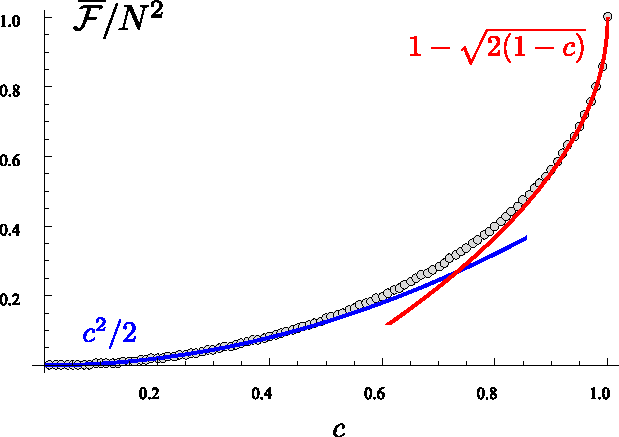
\includegraphics[width=0.7\textwidth]{./figs_Komar2015/Fisher_inf.pdf}
\caption
[Average Fisher information]
{
\label{fig:Fisher_inf}
Average Fisher information as a function of the contrast
$c$ (dots). It is well approximation by $c^2/2$ for $c < 0.6$ and by
$1-\sqrt{2(1-c)}$ for $c > 0.8$ (solid curves).} 
\end{figure}

\subsection{Cram\'{e}r-Rao bound}

The average Fisher information $\overline{\mathcal{F}}$ is a good measure of the
posterior uncertainty of the phase $\phi$, if the prior distribution of the
phase has been previously narrowed down to a small enough interval such that
its posterior is single peaked.
 In case of using the GHZ state, this requires a
very narrow prior to start with: $\phi \in [-\pi/N, +\pi/N]$. In our previous
work, we showed that this is possible by employing the atoms in a scheme using a
series of cascaded GHZ states \cite{Kessler2014}. The Cram\'{e}r-Rao bound on the
expected deviation of the estimated $\phi$ from the true one implies
\bel
	\Delta\phi = \sqrt{\Ev{(\phi_\mathrm{estimate} - \phi_\mathrm{true})^2} }\geq  
	\Big[\nu\overline{\mathcal{F}}\Big]^{-1/2},
\eel
where $\nu$ is the number of independent repetitions of the measurement. We are
going to assume equality to simplify our analysis.


\subsection{Allan-deviation}
The average fractional frequency uncertainty of an atomic clock (with central
frequency $\omega_0$), averaged over a long time period $\tau$, is called
Allan-deviation \cite{Kessler2014},
\bal
	\sigma = \frac{(\Delta\omega)_\tau}{\omega_0} \approx
	\frac{\Delta\phi_t/t}{\omega_0} \frac{1}{\sqrt{\tau/t}}
	\approx
	\frac{1}{\omega_0\sqrt{\tau}}\big[\nu t
	\overline{\mathcal{F}}\big]^{-1/2}\quad\quad
\eal
where $(\Delta \omega)_\tau =
\left|\frac{1}{\tau}\int\d{\tau'}\omega(\tau') - \omega_0\right|$ is the
deviation of the average frequency over time $\tau$, and $\Delta\phi_t$ is
the average deviation of the measured phase (from the true one) in a single
interrogation of length $t$. The $\sqrt{\tau/t}$ factor comes from the number of
independent repetitions of the same, $t$-long, interrogation cycle.

In Ref. \cite{Komar2014}, we showed that $\sigma$ can reach
\bel
	\sigma_\mathrm{ent} \approx \frac{1}{\omega_0 \tau} \frac{8}{\pi}\frac{\sqrt{\log
	N}}{N},
\eel 
if $\tau < \gamma_\mathrm{at}^{-1}/N$, the reduced atomic coherence time, and if
the contrast is perfect, ($c=1$). Using the approximation for
$\overline{\mathcal{F}}\approx N^2 c^2/2$,  and the fact that $\sigma \propto
[\overline{\mathcal{F}}]^{-1/2}\propto c^{-1}$, we can augment this result with
a $c$-dependence, and express the Allan-deviation in the presence of
imperfections as
\bel
	\sigma_\mathrm{ent}^\mathrm{(imperfect)} = \sigma_\mathrm{ent}/c = \frac{1}{c\omega_0
	\tau}\frac{8}{\pi}\frac{\sqrt{\log N}}{N}.
\eel


\subsection{Comparison to non-entangled interrogation}
Using the same number of atoms, $N$, we can arrange a measurement without using
any entanglement. This results in the Allan-deviation of
\bel
\label{eq:sigma_single}
	\sigma_\mathrm{non-ent}(\tau) \approx \frac{1}{\omega_0 \tau\sqrt{N}},\qquad
	\mathrm{if}\quad \tau < 1/\gamma_\mathrm{LO},
\eel
where $\gamma_\mathrm{LO}^{-1}$ is the laser coherence time.
This, representing the standard quantum limit (SQL), is expected to be larger
than the Allan-deviation corresponding to the GHZ state scheme, which is almost
at the Heisenberg limit. The precision gain of the GHZ scheme over the
non-entangled one is
\bel
\label{eq:gain}
	G = \frac{\sigma_\mathrm{non-ent}}{\sigma_\mathrm{ent}/c} =
	(2F_N -1)\frac{\pi}{8}\sqrt{\frac{N}{\log{N}}}.
\eel
Since the fidelity $F_N$ decreases with increasing $N$, there exist an optimal
$N_\mathrm{opt}$, for which the gain $G$ is maximal.

\subsection{Optimal clock network size}
If each clock runs with the optimal setup ($\delta_\mathrm{opt},\,
\omega_\mathrm{opt},\, n_\mathrm{opt}$), then the total error per atom, $E$, is
minimal, and the total fidelity can be written as $F_N =
\left[1+e^{-E_\mathrm{min}N}\right]/2$. Plugging this into \refeq{eq:gain} gives
\bel
	G = e^{-E_\mathrm{min} N} \frac{\pi}{8}\sqrt{\frac{N}{\log N}},
\eel 
which takes its maximum at $N = N_\mathrm{max} \approx \frac{1}{2E_\mathrm{min}}$,
giving $G_\mathrm{max} \approx \frac{\pi}{8}
\left[E_\mathrm{min}\log\left(\frac{1}{2E_\mathrm{min}}\right)\right]^{-1/2}$.
In the meantime the number of atoms at a single clock is given by $ n_\mathrm{opt}$.
As a result the optimal number of clocks becomes 
\bel
	K_\mathrm{opt} \leq \frac{N_\mathrm{max}}{n_\mathrm{opt}} \approx
	\frac{1}{2E_\mathrm{min}n_\mathrm{opt}}.
\eel

On \reffig{fig:K}, we plot $N_{\mathrm{max}}$, $n_\mathrm{opt}$, and
$K_\mathrm{opt}$ as a function of the principle quantum number of the
Rydberg states $\tilde n$.
\begin{figure}[h]
\centering
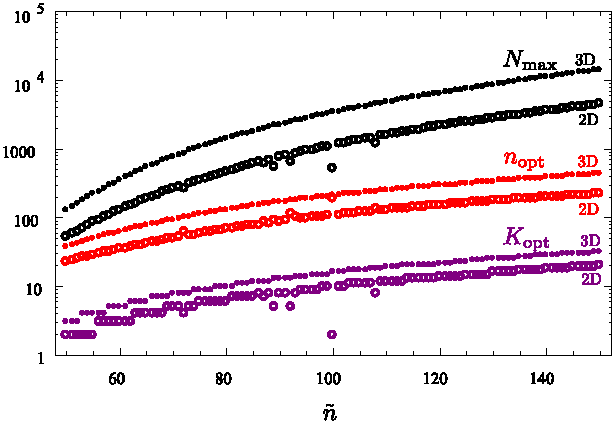
\includegraphics[width=0.8\textwidth]{./figs_Komar2015/NnK_2d3d.pdf}
\caption
[Optimal network size]
{
\label{fig:K}
The optimal total number of entangled atoms in the network $N_\mathrm{max}$ and
the number of atoms at a single clock $n_\mathrm{opt}$ as a function of the principle quantum
number $\tilde n$. The thin dotted lines show the
multiples of $n_\mathrm{opt}$. The optimal number of clocks,
$K_\mathrm{opt} \leq N_\mathrm{max}/n_\mathrm{opt}$ is written on the corresponding
regions of $\tilde n$, for the 2D and 3D setup.}
\end{figure}
For $\tilde n = 120$, we find $N_\mathrm{max} \approx 2500$ (2D) and $\approx
7500$ (3D). Using the $n_\mathrm{opt}$ values from before ($\approx 150$ and
$\approx 300$ ), we find $K_\mathrm{opt} = 14$ and $22$, for 2D and 3D,
respectively.

With the optimal architecture, we can plot the maximal gain $G_\mathrm{max}$
(compared to the non-entangled scheme using the same number of atoms) as a
function of principle quantum number $\tilde n$.
This is shown on \reffig{fig:gain}.
\begin{figure}[h]
\centering
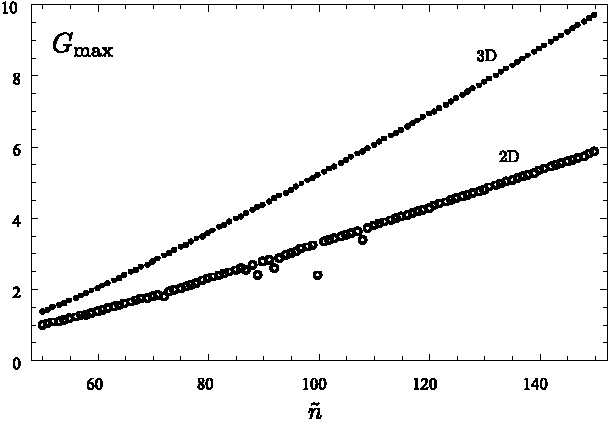
\includegraphics[width=0.8\textwidth]{./figs_Komar2015/gain_2d3d.pdf}
\caption
[Maximal gain over classical schemes]
{
\label{fig:gain}
Maximal gain over the non-entangled scheme provided by the optimal entangled
clock network architecture as a function of principle quantum number of the
Rydberg states $\tilde n$, for the 2D and 3D setup.}
\end{figure}
For $\tilde n = 120$, the gain is $G_\mathrm{max} = 4.3$ (2D) and $6.9$ (3D).


\section{Multiple local ensembles}
Although, in the rest of the paper, we assume that ensembles are separated such
that we need to use photons to generate entanglement between them, one can
imagine employing multiple atomic ensembles in the same vacuum chamber. With
proper optical control, this allows entangling the ensembles by moving a single
Rydberg atom to the vicinity of each ensemble sequentially, such that the its
blockade radius covers one the of clouds entirely.

Disregarding the technical difficulties of trapping multiple atomic ensembles in
the same vacuum chamber, this entangling method has a higher fidelity than the
previous, photon-based, protocol, since it does not suffer from the errors
affecting the photon emission, propagation and detection. We model the
imperfections of this scheme by summing the error terms $\eps_1 + \eps_2 +
\eps_3 + \eps_4 + \eps_5$ only (from Eq.
(\ref{eq:f1}), (\ref{eq:f2}), (\ref{eq:f3}), (\ref{eq:f4}), (\ref{eq:f5})).

In both the 2D and the 3D case the error from the imperfect branching ratio
($e_8$) makes up $30-40\%$ of the total error, and $e_6$ and $e_7$ are
negligible. This translates to a $\sim 30\%$ decrease in total error per atom
($E_\mathrm{one}$), which makes the final gain $G$ about $10\%$ higher.

This means that if the total number of available atoms in a single vacuum
chamber is higher than $n_\mathrm{opt}$, then the best strategy is to create
multiple ensembles of size $n_\mathrm{opt}$ in the chamber, and entangle them with
the above described operation.
The gain is still a factor of $\sim 8$ on top of any classical scheme.


\section{Calculating $\mathrm{Var}(\phi_{j,k})$}
\label{sec:calc_varPhi_jk}
Here, we calculate the variance of 
\bel
	\phi_{j,k} = \frac{\pi\Delta}{\Delta + \Delta_{j,k}} 
	\approx \frac{\pi\Delta}{\Delta_{j,k}}
	= \frac{\pi \hbar \Delta}{C_{12}^{(3)}} |\br_j - \br_k|^3,
\eel
where we assume $\Delta_{j,k} \gg \Delta$ for all $(j,k)$ pairs, 
over an ensemble of $n$ atoms, trapped in a (square or cubic)lattice with
periodicity $a$, uniformly filling a circular 2D (spherical 3D) region of radius
$R$.



\subsection{Calculating $\ev{\phi_{j,k}}$}
Averaging over the cloud of atoms,
\bel
	\ev{\phi_{j,k}} = \frac{\pi\hbar\Delta}{C_{12}^{(3)}} \Ev{|\br_j - \br_k|^3},
\eel
can be approximated by the following integral
\bel
	\approx \frac{\pi\hbar\Delta}{C_{12}^{(3)}} \frac{1}{V^2}\intop_V\d{^\eta
	\br_j}\intop_V\d{^\eta \br_k}|\br_j - \br_j|^3 =
	\frac{\hbar R^3\Delta}{C_{12}^{(3)}} J_1,
\eel
where $\eta = 2,3$,  $V$ is the filled region, of radius $R$, in a (2D or 3D)
lattice, and the integral $J_1$ is
\bal
	J_1^\mathrm{(2D)} &=& \frac{1}{\pi R^7} \intop_0^R \d{r}2\pi r
	\intop_0^{2R}\d{x}S_R(r,x) x^3
	\\
	J_1^\mathrm{(3D)} &=& \frac{9}{16 \pi R^9} \intop_0^R \d{r}4\pi r^2
	\intop_0^{2R}\d{x}A_R(r,x) x^3
\eal
where the new variables are: $x = |\br_j - \br_k|$, $r = |\br_j|$, and we used
the circular (spherical) symmetry of the cloud and the spherical symmetry of the
interaction, to turn the integrals into one dimensional ones. The
weighting factor $S_R(r,x)$ is the length of the segment of a circle of radius
$x$, centered at $r$ distance from the origin that lies inside the 2D cloud of
radius $R$. (See \reffig{fig:circles}).
It can be written as
\bal
\label{eq:S_R}
	S_R(r,x) &=&
	\left\{
	\begin{array}{ll}
		2\pi x &,\, \mathrm{if}\; x < R-r \\ 
		0 &,\, \mathrm{if}\; R+r < x \\
		2x \arccos\left(\frac{x^2 + r^2 - R^2}{2xr}\right) &,\, \mathrm{otherwise}
	\end{array}
	\right.\quad
\eal
\begin{figure}[h]
\centering
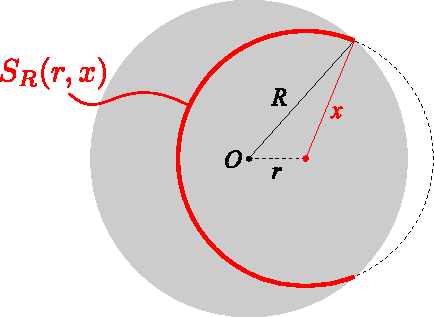
\includegraphics[width=0.45\textwidth]{./figs_Komar2015/circles.pdf}
\caption
[Arc length in a circular cloud]
{
\label{fig:circles}
The length of the circle segment of radius $x$ lying inside the cloud of radius
$R$, $S_R(r,x)$, is between 0 and $2\pi x$ for $R-r < x < R+r$, where $r$ is
the separation between the centers.}
\end{figure}
Similarly, $A_R(r,x)$ is the area of a spherical surface or radius
$x$ centered  $r$ distance from the center of the 3D
cloud located inside the cloud.
It can be written as
\bal
\label{eq:A_R}
	A_R(r,x) &=&
	\left\{
	\begin{array}{ll}
		4\pi x^2 &,\, \mathrm{if}\; x < R-r \\
		0 &, \, \mathrm{if}\; R+r < x\\
		\pi\frac{x}{r}\left[R^2 - (x-r)^2\right] &,\, \mathrm{otherwise}
	\end{array}
	\right.\quad
\eal
Using the explicit expressions of \refeq{eq:S_R} and (\ref{eq:A_R}), we can
write
\bal
	J_1^\mathrm{(2D)} &=& 4\intop_0^1\d{\rho} \rho \left[\intop_0^{1-\rho}\d{\xi}
	\pi \xi^4 
	+\intop_{1-\rho}^{1+\rho}\d{\xi}
	\xi^4\arccos\left(\frac{\xi^2+\rho^2-1}{2\rho\xi} \right)\right]
	\\
	J_1^\mathrm{(3D)} 
	&=& 
	9\pi \intop_0^1\d{\rho}\rho^2 
	\left[
	\intop_0^{1-\rho}\d{\xi}\xi^5
	+
	\frac{1}{4}\intop_{1-\rho}^{1+\rho}\d{\xi}\frac{\xi^4}{\rho}
	\left[1-(\xi-\rho)^2\right]
	\right]	
\eal

which we numerically evaluate and find $J_1^\mathrm{(2D)} = 3.901$, and
$J_1^\mathrm{(3D)} = 4.787$.

\subsection{Calculating $\ev{\phi_{j,k}^2}$}
Similarly, averaging the square is done by evaluating
\bel
	\ev{\phi_{j,k}^2} = \left(\frac{\pi\hbar\Delta}{C_{12}^{(3)}}\right)^2
	\Ev{|\br_j - \br_k|^6},
\eel
which can be express with the integral
\bel
	\!\!\!\approx\left(\frac{\hbar
	R^3\Delta}{C_{12}^{(3)}}\right)^2\!\! \frac{\pi^2}{R^6V^2}\intop_V\d{^\eta
	\br_j}\intop_V\d{^\eta \br_k}|\br_j - \br_j|^3
	= \left(\frac{\hbar
	R^3\Delta}{C_{12}^{(3)}}\right)^2 \!\!\! J_2,
\eel
where
\bal
	J_2^\mathrm{(2D)} &=& \frac{1}{R^{10}}\intop_0^R\d{r}2\pi r \intop_0^{2R}
	\d{x}S_R(r,x) x^6,
	\\
	J_2^\mathrm{(3D)} &=& \frac{9}{16 R^{12}}\intop_0^R\d{r}4\pi r^2 \intop_0^{2R}
	\d{x}A_R(r,x) x^6,
\eal
using the same notation as above. Using the explicit expression of
\refeq{eq:S_R} and (\ref{eq:A_R}), we can write
\bal
	J_2^\mathrm{(2D)} &=& 4\pi\intop_0^1\d{\rho}\rho\left[
	\pi\intop_0^{1-\rho}\d{\xi}\xi^7 
	+ \intop_{1-\rho}^{1+\rho}\d{\xi}\xi^7\arccos\left(\frac{\xi^2 +
	\rho^2 -1}{2\rho\xi}\right)\right]
\eal
\bal
	J_2^\mathrm{(3D)} &=& 9\pi^2\intop_0^1\d{\rho}\rho^2\left[
	\intop_0^{1-\rho}\d{\xi}\xi^8
	+ \frac{1}{4}\intop_{1-\rho}^{1+\rho}\d{\xi}\frac{\xi^7}{\rho}
	\left[1-(\xi-\rho)^2\right]
	\right]
\eal
which we numerically evaluate and find $J_2^\mathrm{(2D)} = 34.54$, and
$J_2^\mathrm{(3D)} = 42.11$.

\subsection{Result for $\mathrm{Var}(\phi_{j,k})$}
The variance in question is
\bel
	\mathrm{Var}(\phi_{j,k}) = \ev{\phi_{j,k}^2} - \ev{\phi_{j,k}}^2
	= \left(\frac{\hbar R^3\Delta}{C_{12}^{(3)}}\right)^2 \left[J_2 - J_1^2\right].
\eel
After plugging in $R = a (n/\pi)^{1/2}$ (for 2D) and $R = a (3n/(4\pi))^{1/3}$
(for 3D), we get
\bal
\label{eq:Var_phi_jk_2D}
	\mathrm{Var}(\phi_{j,k})^\mathrm{(2D)} &=& 0.6233 \, n^3
	\left(\frac{\hbar a^3 \Delta}{C_{12}^{(3)}}\right)^2
	\\
\label{eq:Var_phi_jk_3D}
	\mathrm{Var}(\phi_{j,k})^\mathrm{(3D)} &=& 1.094 \, n^2
	\left(\frac{\hbar a^3 \Delta}{C_{12}^{(3)}}\right)^2
\eal

\section{Calculating $\mathrm{Var}(\psi_j)$}
\label{sec:calc_varPsi_j}
We defined $\psi_j = \sum_{k\neq j} \phi_{j,k}$ in section
\ref{sec:imperfect_blockade}. Here we evaluate its variance.

\subsection{Calculating $\ev{\psi_j}$}
The average over the 2D (or 3D) cloud can be written as
\bal
	\ev{\psi_j} = \Ev{\sum_k \phi_{j,k}} = \frac{1}{n}\sum_j\sum_k \phi_{j,k} =
	n\ev{\phi_{j,i}},
\eal
which we evaluated in section \ref{sec:calc_varPhi_jk}. Using the notation used
there, we can write
\bel
	\ev{\psi_j} = n\frac{\hbar R^3 \Delta}{C_{12}^{3}} J_1. 
\eel

\subsection{Calculating $\ev{\psi_j^2}$}
The average of the square can be written as
\bel
	\ev{\psi_j^2} = \frac{1}{n}\sum_j\left(\sum_{k\neq j}\phi_{j,k}\right)^2 = 
	\frac{n^2}{V^3} \intop_V\d{^\eta\br_j}\left(\intop_V\d{^\eta\br_k}
	\phi_{j,k}\right)^2,
\eel
where $\eta = 2,3$, and $V$ is the circular (in 2D) or spherical (in 3D) region
filled with $n$ atoms, homogeneously. After plugging in the expression for
$\phi_{j,k}$ and using the same notation as in section \ref{sec:calc_varPhi_jk},
we write
\bel
	\ev{\psi_j^2} = n^2 \left(\frac{\hbar R^3\Delta}{C_{12}^{3}}\right)^2 J_3,
\eel
where
\bal
	J_3^\mathrm{(2D)} &=& \frac{1}{\pi R^{12}}\intop_0^R\d{r}2\pi r
	\left(\intop_0^{2R}\d{x}S_R(r,x) x^3\right)^2,
	\\
	J_3^\mathrm{(3D)} &=& \frac{27}{64\pi R^{15}}\intop_0^R\d{r}4\pi r^2
	\left(\intop_0^{2R}\d{x}A_R(r,x) x^3\right)^2.
\eal
Using the explicit expressions from \refeq{eq:S_R} and (\ref{eq:A_R}) gives
\bal
	J_3^\mathrm{(2D)} &=& 
	8\intop_0^1\d{\rho}\rho
	\left[
		\left(\pi\intop_0^{1-\rho}\d{\xi}\xi^4\right)^2
	\right.
	\nonumber\\
	&&+
		2\left(\pi\intop_0^{1-\rho}\d{\xi}\xi^4\right)
		\left(\intop_{1-\rho}^{1+\rho}\d{\xi}\xi^4\arccos
		\left(\frac{\xi^2+\rho^2-1}{2\rho\xi}\right)\right)
	\nonumber\\
	&&+
	\left.
		\left(\intop_{1-\rho}^{1+\rho}\d{\xi}\xi^4\arccos
		\left(\frac{\xi^2+\rho^2-1}{2\rho\xi}\right)\right)^2
	\right]
\eal
\bal
	J_3^\mathrm{(3D)} &=& 
	27\pi^2\intop_0^1\d{\rho}\rho^2
	\left[
		\left(\intop_0^{1-\rho}\d{\xi}\xi^5\right)^2
	\right.
	\nonumber\\
	&&+
		2\left(\intop_0^{1-\rho}\d{\xi}\xi^5\right)
		\left(\intop_{1-\rho}^{1+\rho}\d{\xi}\frac{1}{4}\frac{\xi^4}{\rho}
		\left[1-(\xi-\rho)^2\right] \right) \nonumber\\
	&&+
	\left.
		\left(\intop_{1-\rho}^{1+\rho}\d{\xi}\frac{1}{4}\frac{\xi^4}{\rho}
		[1-(\xi-\rho)^2] \right)^2
	\right]
\eal
We evaluate these numerically and find $J_3^\mathrm{(2D)} = 17.81$, and 
$J_3^\mathrm{(3D)} = 25.16$.

\subsection{Result for $\mathrm{Var}(\psi_j)$}
Now, the variance in question can be written as
\bel
	\mathrm{Var}(\psi_j) = \Ev{\psi_j^2} - \ev{\psi_j}^2 = n^2
	\left(\frac{\hbar R^3 \Delta}{C_{12}^{(3)}}\right)^2 \left[J_3 - J_1^2\right].
\eel
After plugging in $R = a (n/\pi)^{1/2}$ (for 2D) and $R = a (3n/(4\pi))^{1/3}$
(for 3D), we get
\bal
	\mathrm{Var}(\psi_j)^\mathrm{(2D)} 
	&=&
	0.08359\, n^5 \left(\frac{\hbar a^3 \Delta}{C_{12}^{(3)}}\right)^2 
	\\
	\mathrm{Var}(\psi_j)^\mathrm{(3D)} 
	&=&
	0.1277\, n^4 \left(\frac{\hbar a^3 \Delta}{C_{12}^{(3)}}\right)^2 
\eal

\section{Calculating $\mathrm{Var}(\Delta_j)$}
\label{sec:calc_varDelta_j}
Here, we calculate the variance of $\Delta_j = -\sum_{k\neq
j}\frac{\Omega^2}{4(\Delta_{j,k} + \Delta)}\approx -\sum_{k\neq
j}\frac{\Omega^2}{4\Delta_{jk}}$ in case of $\Delta \ll \mathrm{min}\,
\Delta_{j,k}$, for an ensemble of $n$ atoms, trapped in a lattice with
periodicity $a$, uniformly filling a circular 2D (spherical 3D) region of radius
$R$.
We assume a van der Waals interaction, $\Delta_{j,k} = \frac{C_{11}^{(6)}}{\hbar |\br_j
- \br_k|^6}$ between pairs of atoms at $\br_j$ and $\br_k$.

\subsection{Calculating $\ev{\Delta_j}$}
Averaging over the ensemble of atoms,
\bel
	\ev{\Delta_j} = \frac{1}{n}\sum_j \Delta_j =
	\left(-\frac{\hbar\Omega^2}{4 C_{11}^{(6)}}\right) \frac{1}{n}\sum_j
	\sum_{k\neq j}|\br_j - \br_k|^6
\eel
can be approximated with the following integral
\bal
	\ev{\Delta_j}
	&\approx &
	\left(-\frac{\hbar\Omega^2}{4 C_{11}^{(6)}}\right) \frac{n}{V^2} \intop_V
	\d{^\eta\br_j}\intop_V\d{^\eta\br_k} |\br_j - \br_k|^6\quad
	\\
	&=& - n \frac{\hbar\Omega^2 R^6}{C_{11}^{(6)}} I_1,
\eal
where $\eta = 2$ or $3$, and $V$ is the filled region, of radius $R$, of the (2D
or 3D) lattice, and $I_1$ is the following integral,
\bal
\label{eq:I_1_2D}
	I_1^\mathrm{(2D)} &=& 
	\frac{1}{(2\pi)^2 R^{10}} \intop_0^R \d{r} 2\pi r \intop_0^{2R}\d{x}
	S_R(r,x) x^6,
	\\
\label{eq:I_1_3D}
	I_1^\mathrm{(3D)} &=&
	\frac{9}{64 \pi^2 R^{12}} \intop_0^R\d{r} 4\pi r^2 \intop_0^{2R}\d{x}A_R(r,x)
	x^6,
\eal 
where we used the same transformation as in section
\ref{sec:calc_varPhi_jk}, and $S_R(r,x)$ and $A_R(r,x)$ are given by
\refeq{eq:S_R} and (\ref{eq:A_R}).

Now, we can
express $I_1$, in terms of the dimensionless variables $\rho = r/R$, $\xi = x/R$, as
\bal
	&&I_1^\mathrm{(2D)} = \intop_0^1\d{\rho} \rho\left[\intop_0^{1-\rho}\d{\xi} 
	\xi^7 + \frac{1}{\pi}\intop_{1-\rho}^{1+\rho}\d{\xi}  \xi^7
	\arccos\left(\frac{\xi^2 + \rho^2 -1}{2\xi \rho}\right)
	\right]
	\nonumber\\
	&&I_1^\mathrm{(3D)} = \frac{9}{4}\intop_0^1\d{\rho}
	\rho^2\left[\intop_0^{1-\rho}\d{\xi} \xi^8 +
	\intop_{1-\rho}^{1+\rho}\d{\xi}  \xi^8 \frac{1-(\xi-\rho)^2} {4\xi
	\rho} \right]
	\nonumber
\eal
which we evaluate numerically and find $I_1^\mathrm{(2D)} = 0.875$, and
$I_1^\mathrm{(3D)} = 1.067$.

\subsection{Calculating $\ev{\Delta_j^2}$}
The average of $\Delta_j^2$ can be written as
\bel
	\ev{\Delta_j^2} = \frac{1}{n}\sum_j\Delta_j^2 =
	\left(\frac{\hbar\Omega^2}{4 C_{11}^{(6)}}\right)^2 \frac{1}{n}\sum_j
	\left(\sum_{k\neq j} |\br_j - \br_k|^6\right)^2.
\eel
Similarly to the calculation of $\ev{\Delta_j}$, we can approximate the sums
with integrals and write
\bel
	\ev{\Delta_j^2} = \left(n \frac{\hbar\Omega^2 R^6}{C_{11}^{(6)}}\right)^2 I_2,
\eel
where $I_2$ takes the following forms
\bal
	I_2^\mathrm{(2D)} &=& \frac{1}{16\pi^3 R^{18}} \intop_0^R\d{r}2\pi r
	\left(\intop_0^{2R}\d{x}S_R(r,x)x^6\right)^2
	\\
	I_2^\mathrm{(3D)} &=& \frac{27}{256 \pi^3 R^{21}} \intop_0^R\d{r}4\pi r^2 
	\left(
	\intop_0^{2R}\d{x}A_R(r,x) x^6
	\right)^2
\eal
in the two cases.

After plugging in the explicit expressions of $S_R(r,x)$ and $A_R(r,x)$, we can
express $I_2$ in terms of the dimensionless variables $\rho = r/R$, $\xi = x/R$, as
\bal
	I_2^\mathrm{(2D)} &=&
	\frac{1}{2}\intop_0^1\d{\rho} \rho
	\left[\left(\intop_0^{1-\rho}\d{\xi} \xi^7\right)^2 \right. 
	\nonumber\\
	&& +
	\frac{2}{\pi}\left(\intop_0^{1-\rho}\d{\xi}\xi^7
	\right) \left(\intop_{1-\rho}^{1+\rho} \d{\xi} \xi^7 \arccos\left(\frac{\xi^2 +
	\rho^2 -1}{2\xi\rho}\right)\right) \nonumber\\
	&& \left. + \frac{1}{\pi^2}
	\left(\intop_{1-\rho}^{1+\rho} \d{\xi} \xi^7 \arccos\left(\frac{\xi^2 +
	\rho^2 -1}{2\xi\rho}\right)\right)^2 \right],
\label{eq:I_2_2D}
\eal
\bal
	I_2^\mathrm{(3D)} &=&
	\frac{27}{16}\intop_0^1\d{\rho}\rho^2\left[
	\left(\intop_0^{1-\rho}\d{\xi}\xi^8\right)^2 
	\right.
	\nonumber \\
	&&+ \frac{1}{2}\left(\intop_0^{1-\rho}\d{\xi}\xi^8\right)
	\left(\intop_{1-\rho}^{1+\rho}\d{\xi} \frac{\xi^7}{\rho}[1 -
	(\xi-\rho)^2]\right) \nonumber \\
	&&\left. + \frac{1}{16}
	\left(\intop_{1-\rho}^{1+\rho}\d{\xi}\frac{\xi^7}{\rho}[1-(\xi
	-\rho)^2]\right)^2 \right]
\label{eq:I_2_3D}
\eal
which we evaluate numerically and find $I_2^\mathrm{(2D)} = 1.146$, and
$I_2^\mathrm{(3D)} = 1.474$

\subsection{Result for $\mathrm{Var}(\Delta_{j})$}
Using the results above, we write the variance of $\Delta_j$ as
\bel
	\mathrm{Var}(\Delta_j) = \ev{\Delta_j^2} - \ev{\Delta_j}^2 = n^2
	\left(\frac{\hbar\Omega^2 R^6}{C_{11}^{(6)}}\right)\left[I_2 -
	(I_1)^2\right].
\eel 
Instead of $R$, we can also write it, in terms of the lattice constant
$a$, and the total number of atoms $n$, as
\bal
\label{eq:varDelta_j_2D}
	\mathrm{Var}(\Delta_j)^\mathrm{(2D)} &=& \frac{0.380}{\pi^6} n^8
	\left(\frac{\hbar \Omega^2a^6}{C_{11}^{(6)}}\right)^2,
	\\
\label{eq:varDelta_j_3D}
	\mathrm{Var}(\Delta_j)^\mathrm{(3D)} &=& \frac{81}{128}\frac{0.336}{\pi^4} n^6
	\left(\frac{\hbar \Omega^2a^6}{C_{11}^{(6)}}\right)^2,
\eal
where we used that $R^2 \pi = n a^2$ (in 2D) and $4\pi R^3/3 = na^3$ (in 3D).

